\chapter{Linux On Cyclone V}
\label{ch:linuxoncyclonev}

We have downloaded the system image from the Altera website and put it on the SD card with Win32DiskImager.exe.\\
We connected with Putty and it showed that Linux booted up successfully.

\section{Debug on Linux}
\begin{figure}[h]
	\centering		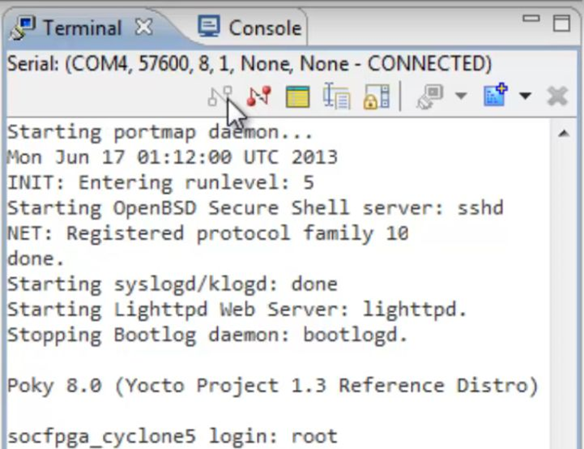
\includegraphics[width=0.8\textwidth]{img/debugterminal}
	\caption{Debug terminal}
    	\label{fig:debugterminal}
\end{figure}

To debug on Linux with the Cyclone V was needed an Eclipse based environment called DS-5 debugger included in the intelFPGA software.\\
We connected it to the serial and the boot was showed in its terminal panel.
\clearpage

\begin{figure}[h]
	\centering		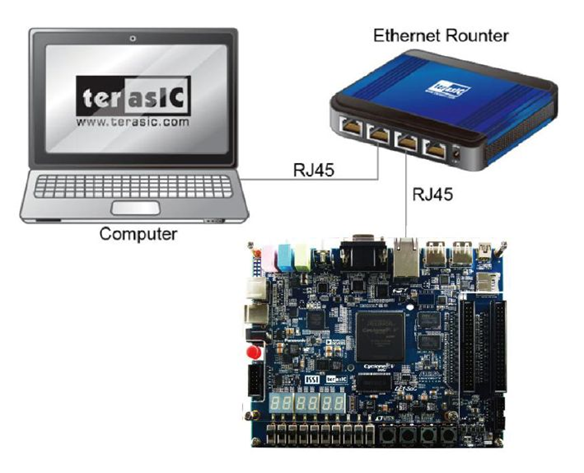
\includegraphics[width=0.8\textwidth]{img/routerconf}
	\caption{Router connection}
    	\label{fig:routerconf}
\end{figure}

As told in “My First HPS guide provided by Altera, a router was needed to connect the PC with the board via Ethernet.\\
However the router was only needed for its DHCP protocol, so we manually configured the board with ifconfig eth0 $192.168.1.4$ netmask $255.255.255.0$ up in the terminal.\\
In Windows in LAN settings we configured the network as in the image.\\
We executed the ping command and it worked.
\clearpage

\begin{figure}[h]
	\centering		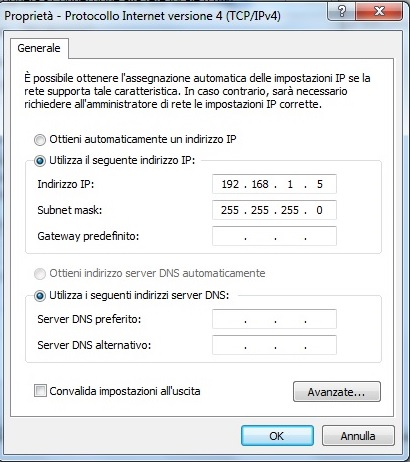
\includegraphics[width=0.6\textwidth]{img/internetprop}
	\caption{Internet properties}
    	\label{fig:internetprop}
\end{figure}

\begin{figure}[h]
	\centering		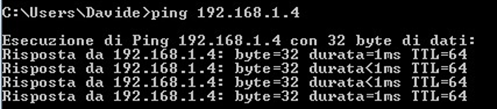
\includegraphics[width=0.8\textwidth]{img/ping}
	\caption{Connection test}
    	\label{fig:ping}
\end{figure}

\clearpage
We executed the following commands to activate the ssh protocol.\\
Then in the remote system panel  we defined an ssh only connection with host name the board IP and a connection name. We opened it and it requested a password, but was only necessary to write root in the host name to gain the access.\\

\begin{figure}[h]
	\centering		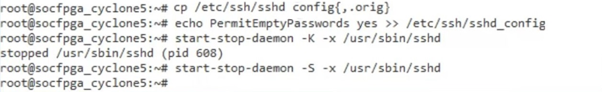
\includegraphics[width=0.6\textwidth]{img/comand}
	\caption{Commands}
    	\label{fig:comand}
\end{figure}


Once established a connection to test the debug function, we opened a software made by Altera: intelFPGA-embedded-examples-software-Altera-SoCFPGA-Blinking-LED-Linux-GNU.tar.gz\\
When we tried to build the project an error showed up due to a licensing problem:


\begin{figure}[h]
	\centering		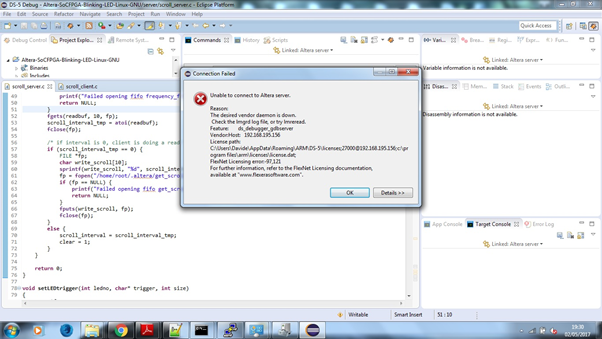
\includegraphics[width=0.8\textwidth]{img/licenseerror}
	\caption{License error}
    	\label{fig:licenseerror}
\end{figure}

Once downloaded the licence, it builded the project. Then we created a new configuration in the panel “Debug configuration” for the application server side following these steps:

\clearpage
\begin{figure}[h]
	\centering		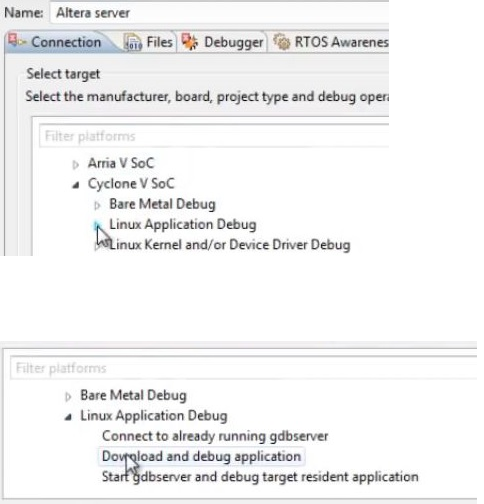
\includegraphics[width=0.8\textwidth]{img/downloadonborad}
	\caption{Download on borad}
    	\label{fig:downloadonborad}
\end{figure}

\begin{figure}[h]
	\centering		
\includegraphics[width=0.8\textwidth]{img/downloadsucces}
	\caption{Download success}
    	\label{fig:downloadsucces}
\end{figure}

Same steps for the client side but changing the following parameters.


\begin{figure}[h]
	\centering		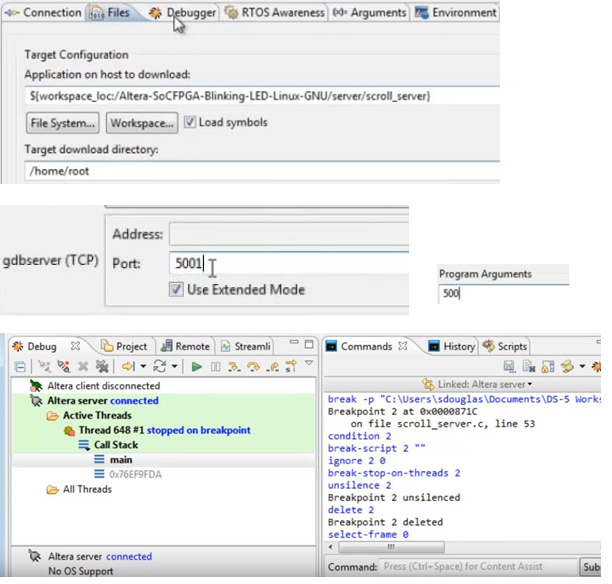
\includegraphics[width=0.8\textwidth]{img/setting}
	\caption{Settings}
    	\label{fig:setting}
\end{figure}

Click on Altera server and start debug.

\begin{figure}[h]
	\centering		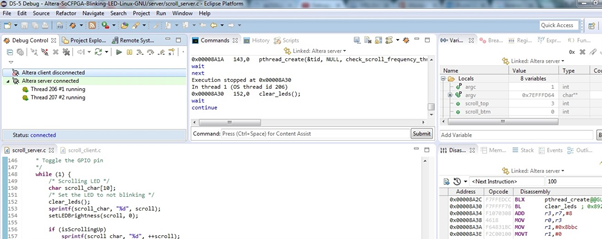
\includegraphics[width=0.8\textwidth]{img/debug}
	\caption{Debug}
    	\label{fig:debug}
\end{figure}















